\chapter{Data Engineering Workflow}

In the second chapter, a detailed overview of the workflow for data engineering is presented. This overview covers important areas of data management, processing, storage and governance. Beginning with an examination of the dimensions s of data quality — its correctness, completeness, consistency, timeliness and uniqueness — the chapter moves on to discuss how to guarantee reliable and valuable data assets.

Following that, the chapter explores data ingestion, processing and storage processes. In it, several data pipeline designs are discussed and a comparison is made between ETL (Extract, Transform, Load) and ELT (Extract, Load, Transform) techniques. Additionally, the benefits and implementation scenarios of each strategy are highlighted.

A considerable section of the chapter is devoted to the discussion of data storage systems, which includes an explanation of the functions that data warehouses, data lakes and NoSQL databases play in contemporary data management. In managing big amounts of different data types and the need for scalability, performance and flexibility.

Additionally covered in this chapter are important facets of data security and governance, including access control techniques, encryption techniques and the difficulties presented by changing legal requirements. It discusses cutting edge data management technologies and methods, such as the use of ethical AI techniques and machine learning for data quality management.

Data integration, serving and the value of monitoring and maintenance in guaranteeing the seamless functioning of data pipelines are covered in the last section. Throughout, the book offers practical examples and addresses the difficulties and possible fixes in putting into practice efficient data engineering techniques.

With its emphasis on its vital role in allowing data-driven decision-making and insights across many sectors, this thorough introduction provides a basis for comprehending the complicated terrain of contemporary data engineering.

\section{Data Quality Dimensions}

\textbf{Data quality dimensions} — quality and usability of data within a data pipeline.

Before diving into data processing frameworks, it should be clarified on the basis of what data quality is assessed. This subchapter focuses only on 5 data quality dimensions that are the most related to the thesis. However, in the cited paper, there are teens of dimension. Also, it could have been a lot to say about data validation, profiling, cleansing, enrichment, transformations and frameworks, but this is beyond the scope of this master thesis (\cite{andrewblackDimensionsDataQuality2020})\footnotemark[19].

\textbf{Accuracy} — how well data represents reality. It measures the proximity of how close the values in the data are in comparison to the prediction. Inaccurate data may cause incorrect analyses, flawed decision-making and unreliable insights. An excellent example would be a customer database. The recorded addresses and contact information have to be accurate and up to date (\cite{andrewblackDimensionsDataQuality2020})\footnotemark[19].

\textbf{Completeness} — the amount of information available for analysis. It makes sure that the dataset is not corrupted and/or doesn't have any missing values, fields or records. If the information is not complete, it can make it hard to analyze and give wrong or biased results. For example, in a sales transaction dataset, making sure that all fields, such as customer ID, product ID, quantity and price, are filled in for each transaction (\cite{andrewblackDimensionsDataQuality2020})\footnotemark[19].

\textbf{Consistency} — keeping data consistent across different sources, systems and time frames. This makes sure that information is presented in a standard way and follows certain rules for the business. Inconsistent data can lead to confusion, errors and problems when integrating and analyzing data. One way to avoid confusion and make data easier to understand is to use a standard date format called ISO8601 "YYYY-MM-DD" across all data sources (\cite{andrewblackDimensionsDataQuality2020})\footnotemark[19].

\textbf{Timeliness} — gauges how current and easily available data is when it comes time for analysis or decision-making. It guarantees current data that accurately depicts the most recent status of the people or events it represents. Outdated or stale data might result in wrong conclusions and suboptimal decisions. One such system may be a real-time fraud detection system, which would guarantee that transaction data is processed and analyzed in near-real time to spot and stop fraudulent activity early on (\cite{andrewblackDimensionsDataQuality2020})\footnotemark[19].

\textbf{Uniqueness} —  there are no duplicates in a set of data. It guarantees that every record or entity is distinct and consistent. Duplicate information can skew analysis results, consume storage space and lead to incorrect aggregations. In a CRM system, one can use deduplication techniques to find and combine duplicate customer records using unique identifiers or matching criteria (\cite{andrewblackDimensionsDataQuality2020})\footnote[19]{\fullcite{andrewblackDimensionsDataQuality2020}}.

\section{Data Ingestion}

According to (\cite{Kona2023LeveragingSA})\footnotemark[16] \textbf{data ingestion}, for short \textbf{DI} can be defined as process of collecting and importing data from various sources into a data storage system or processing pipeline. This means getting information from different places — like databases, files, streaming platforms and IoT devices — and using them to analyze it (\cite{Kona2023LeveragingSA})\footnote[16]{\fullcite{Kona2023LeveragingSA}}.

\textbf{DI} frequently handles large volumes of data generated at high speeds, such as real-time streaming data or high-throughput transactional systems. Processing and ingesting such data necessitate scalable \textbf{DI} frameworks. The data can appear in multiple formats: structured (e.g., CSV, JSON), semi-structured (e.g., XML, log files) or unstructured (e.g., text, images, videos). \textbf{DI} systems must tackle these varying formats effectively to extract useful information. Moreover, these data pipelines must be failure-resilient and uphold data reliability, maintaining stability against network disruptions, system failures and data inconsistencies without losing essential data or compromising its integrity (\cite{Kona2023LeveragingSA})\footnotemark[16].

\textbf{Batch Ingestion} involves gathering and importing data at regular intervals into the system. Apache Spark is an example of a distributed processing framework that facilitates batch ingestion, handling large datasets in parallel across a cluster of machines. \textbf{Real time streaming} deals with capturing and processing data as it arrives, enabling near-real time analysis and decision-making. These pipelines can be built with tools like \textbf{Apache Kafka}, \textbf{Apache Flink} or \textbf{Akka Streams} (\cite{Kona2023LeveragingSA})\footnotemark[16].

\section{Data Processing}

Getting raw data from a lot of different sources, both inside and outside the company, is the first step in \textbf{data processing}. From transactional databases and operational systems to online logs, social media feeds and Internet of Things sensor networks, these sources may make up a wide variety of information. Due to the fact that the data may be structured, semi-structured or unstructured, it is necessary to have a robust and scalable ingestion framework that is able to manage a variety of data formats and volumes. Data engineers need to come up with and set up efficient ways to get this data out of storage and into a central repository or data lake so it can be processed further (\cite{tomeDataEngineeringScala2024})\footnote[10]{\fullcite{tomeDataEngineeringScala2024}}.

There are a lot of problems with \textbf{raw data}, — like missing values, duplicates, inconsistencies and errors — which can have a big effect on the quality and reliability of analysis that comes after. The goal of the data cleaning phase is to find and fix these problems. It does this by removing duplicate data, dealing with missing values by adding them or deleting them, changing the data type and finding and fixing outliers. This process makes sure that the data meets quality standards that have already been set and is ready to be transformed and analyzed (\cite{tomeDataEngineeringScala2024})\footnotemark[10].

Following the completion of the data cleaning and validation processes, it is then subjected to a transformation process in order to be converted into a format that is optimized for analysis and storage. Data normalization, aggregation, joining data from different sources, feature engineering and data enrichment are some of the tasks that may be done at this stage. The changed data is usually organized in a denormalized or dimensional format, which makes it easier to query and analyze. When designing and putting these transformation pipelines into action, data engineers need to be very careful to think about things like performance, scalability and maintainability (\cite{tomeDataEngineeringScala2024})\footnotemark[10].

Scientists and data analysts can use the processed and changed data in a variety of ways to find insights and help people make decisions based on data. This could include things like data mining, machine learning, statistical analysis and data visualization. These people are closely involved with data engineers, who make sure that the processed data meets their needs and can be easily added to their analytical workflows (\cite{tomeDataEngineeringScala2024})\footnotemark[10].

After the data has been processed and converted, the last step in the data processing process is to store the data in a format that is optimized for querying and for usage in the future. Depending on the needs of the business, this usually means putting the data into data warehouses, data lakes or \textbf{NoSQL} systems. Data engineers are responsible for designing and implementing storage schemas, indexing algorithms and partitioning approaches in order to guarantee optimum performance, scalability and cost-efficiency for analytical workloads they are responsible for (\cite{tomeDataEngineeringScala2024})\footnote[10]{\fullcite{tomeDataEngineeringScala2024}}.

\section{Data Storage Systems}

People in the business world today think of data as the energy that keeps companies going. Companies nowadays are aware that data plays an essential part in their business intelligence systems, which enables them to make choices based on accurate information and to keep a competitive edge in their particular industries (\cite{Nambiar2022AnOO})\footnote[20]{\fullcite{Nambiar2022AnOO}}. The term "big data" is widely used to refer to the huge amounts of data that are produced, collected and processed by businesses. Managing and studying this data well is necessary to get useful insights and help people make decisions based on data (\cite{Nambiar2022AnOO})\footnotemark[20]. Traditional ways of storing data aren't able to keep up with the huge amounts and types of data that are being created. It can be hard and complicated to deal with and look at the huge amount and variety of "big data." A company can find useful information that helps shape its business plans, though, if it knows how to use and benefit from its huge data collection (\cite{Nambiar2022AnOO})\footnotemark[20]. To deal with these problems, businesses need data storing options that are both efficient and flexible. For the purpose of storing and managing large amounts of data, data warehouses and data lakes have become more popular as data management systems (\cite{Nambiar2022AnOO})\footnotemark[20].

Both\textbf{ data warehouses (DW)} and \textbf{data lakes (DL)} are centralized repositories that are used for the purpose of storing and managing the data used by a business (\cite{Nambiar2022AnOO})\footnotemark[20]. Although there are some parallels between \textbf{DW} and \textbf{DL}, there are also differences between them in terms of their properties and applications. In addition to this, they possess unique qualities that make them suited for a variety of data storage and analysis applications (\cite{Nambiar2022AnOO})\footnotemark[20]. \textbf{DW} saves data in an ordered and organized way, using predefined schemas. They are made for organized data and are built for quick analysis and queries. \textbf{DL}, on the other hand, saves data in its original state, which means that structured, semi-structured and unstructured data can all be stored (\cite{Nambiar2022AnOO})\footnotemark[20]. Another thing is how efficient it is. A relational model has problems with scaling, which means that as the amount of data grows, speed drops quickly. As an answer, a new data model was used. \textbf{NoSQL} databases, like document stores, graph databases, key-value stores and column-oriented databases, were made as replacements to relational databases. They make it easier to handle big data by giving you more scalability, flexibility and speed (\cite{Nayak2013TypeON})\footnote[21]{\fullcite{Nayak2013TypeON}}.

The basis for storing, managing and accessing data at different stages of the pipeline is provided by data storage systems, which play a significant role in the pipeline-based data management system. The \textbf{scalability factor} is very important for showing how important these systems are. \textbf{Data storage} systems need to be able to scale horizontally to meet the growing storage needs as data amounts continue to grow at an exponential rate. Distributed storage options like Amazon S3, Apache Hadoop HDFS and others are made to scale by adding more nodes to the cluster. This makes it possible to handle very large datasets quickly. Even in the event that the hardware fails, these systems include fault tolerance and data replication procedures to guarantee the availability and longevity of the data contained inside them. Scalable data storage systems also allow the creation of data pipelines that can meet the ever-growing needs of big data applications. This makes it easier to store and analyze \textbf{terabytes or petabytes of data}. It is very important to be able to flexibly \textbf{scale storage space} without any downtime or performance problems in order to keep performance and reliability high while dealing with growing data amounts and complexity in data flows (\cite{Nambiar2022AnOO})\footnote[20]{\fullcite{Nambiar2022AnOO}}.

\subsection{The Role and Challenges Associated with Storing}

It is during \textbf{ingestion phase} that data storage systems receive data from a variety of sources, such as databases, files, APIs and streaming services. They have to keep track of the huge amount of data and how quickly it moves so that storing is reliable and effective. At this stage, it's hard to deal with scalability because storage systems need to \textbf{grow to hold more data without losing speed or data integrity}. Distributed storage systems like Amazon S3 and Apache Hadoop HDFS are made to grow horizontally by adding more nodes to the cluster. This lets big data to be stored and processed (\cite{Nambiar2022AnOO})\footnotemark[20].

During the \textbf{processing stage}, data storage systems are both the source and the destination for transformations and calculations that are made on data. They need to make it easy to get to saved data quickly so that data processing tools can get information and change it effectively. At this point, performance is vital because \textbf{storage systems need to be able to handle large amounts of data quickly and with low latency}. By spreading data and calculations across many nodes in the cluster, distributed storage systems and parallel processing tools like Apache Spark make it possible to work with big datasets  (\cite{Nambiar2022AnOO})\footnotemark[20].

Another big problem with storing and handling a large scale data is making sure that \textbf{the data is consistent}. When many systems and users are viewing and changing the data at the same time, it is paramount to make sure that it is consistent and correct. To keep data consistent, data store systems need to have ways to do it. For example, \textbf{ACID (Atomicity, Consistency, Isolation and Durability)} \textbf{traits} in standard databases or eventual \textbf{consistency models} in distributed systems are two examples. Data splitting, replication and versioning are all techniques that help keep data consistent and allow for fault tolerance in case of breakdowns or network partitions (\cite{Nambiar2022AnOO})\footnotemark[20].

During the \textbf{data serving phase}, data storage systems are what send processed and aggregated data to users and apps further downstream. They need to be able to query and retrieve data quickly and easily, often in real time or near real time. At this stage, \textbf{scalability and speed are vital} due to the fact data storing systems need to be able to handle a lot of queries at the same time and return answers with low latency. Distributed databases, including \textbf{Apache Cassandra} and \textbf{Apache HBase}, are intended to offer high-performance data serving capabilities that are both scalable and performant, thereby facilitating the rapid access to large datasets (\cite{Nambiar2022AnOO})\footnotemark[20].

\subsection{Types of Data Storage Systems}

\textbf{Data warehouses} are centralized repositories that are used for the purpose of storing and managing massive amounts of structured data that originate from a variety of sources. As a result of their ability to enable complicated queries, data processing and reporting, they make it possible for enterprises to acquire useful insights from their data (\cite{Nambiar2022AnOO})\footnote[20]{\fullcite{Nambiar2022AnOO}}.

\begin{enumerate}
    \item A \textbf{schema-on-write method} is what they usually use. This means that the data structure is set up front and data is changed and checked before it is put into the warehouse. This makes sure that the data is correct and consistent because it follows a set format (\cite{Nambiar2022AnOO})\footnotemark[20];
    \item Data warehouses are designed to handle \textbf{Online Analytical Processing (OLAP)} tasks like complicated searches, data consolidation and multiple analysis. They have features like sorting, splitting and materialized views that make it easier to query and analyze big datasets quickly (\cite{Nambiar2022AnOO})\footnotemark[20];
    \item They are made to \textbf{handle complicated queries} that involve joining multiple tables, collecting data and doing math. They have query tools that are built on SQL and support advanced query optimization methods to make sure that queries run quickly. Amazon Redshift, Google BigQuery and Snowflake are all types of data centers (\cite{Nambiar2022AnOO})\footnotemark[20].
\end{enumerate}

Another part of data storage systems are \textbf{data lakes}. They let companies use the power of big data analytics by giving them a central place to store huge amounts of raw, unstructured and semi-structured data from different sources (\cite{Nambiar2022AnOO})\footnote[20]{\fullcite{Nambiar2022AnOO}}.

\begin{enumerate}
    \item The way that data lakes and data warehouses handle schemas is different. A schema-on-write method is used in data warehouses, while a \textbf{schema-on-read} method is used in data lakes. In other words, data that is put into a data lake is kept in its original form, without a model that has already been set up. The schema is used when the data is viewed and handled, so it can be changed as the needs of the data change (\cite{Nambiar2022AnOO})\footnotemark[20];
    \item \textbf{Different types of data} can be stored in data lakes. This includes structured data (like CSV and JSON), semi-structured data (like XML and log files) and unstructured (like pictures and videos). Because of this, businesses can get information from a variety of places, such as social media sites, Internet of Things (IoT) devices and clickstream datasets (\cite{Nambiar2022AnOO})\footnotemark[20];
    \item Data lakes are a way to \textbf{store large amounts of data for a low cost}. In order to achieve scalability, robustness and cost effectiveness, they make use of cloud services such as Amazon S3 and Azure Data Lake Storage, as well as distributed storage solutions such as Apache Hadoop HDFS. The data can be stored on hardware or in the cloud and these systems make sure that it is always available. Apache Hadoop HDFS, Amazon S3 and Azure Data Lake Storage are all well-known examples of data lakes (\cite{Nambiar2022AnOO})\footnotemark[20].
\end{enumerate}

\textbf{NoSQL databases} effective handling of semi-structured and unstructured data has made them quite popular in recent years. Because they provide a scalable and versatile substitute for conventional relational databases, they are ideal for managing the wide range of quickly expanding data needs of contemporary data pipelines (\cite{Nayak2013TypeON})\footnote[21]{\fullcite{Nayak2013TypeON}}.

\begin{enumerate}
    \item \textbf{Schema-less} or \textbf{schema-flexible} databases enable data to be stored without a specified schema. This flexibility makes it possible to quickly design and iterate data-driven applications and to easily accommodate changing data structures (\cite{Nayak2013TypeON})\footnotemark[21];
    \item Because they are \textbf{designed to grow horizontally}, NoSQL databases may have data spread across many cluster nodes. Because they provide low latency and excellent speed for read and write operations, they are appropriate for managing big data volumes and high-throughput applications (\cite{Nayak2013TypeON})\footnotemark[21];
    \item Among the \textbf{data models supported by NoSQL databases are key-value, document, column-family and graph}. Every data model offers many methods of data organization and querying and is designed for certain use cases. NoSQL databases include, for instance, Apache Cassandra, MongoDB and Apache HBase. (\cite{Nayak2013TypeON})\footnote[21]{\fullcite{Nayak2013TypeON}}.
\end{enumerate}

\section{Data Integration}

Many sources data are merged into a single viewpoint or format in data integration. It means changing data architecture, resolving contradictions and ensuring that data is consistent and of high quality among many systems.

Generally speaking, \textbf{data sources are heterogeneous}, meaning that data often resides in numerous systems — such as databases, files, APIs and streaming platforms — with various schemas, formats and access mechanisms. Managing many data formats, protocols and APIs is necessary to combine data from several unrelated sources. Additionally possible are duplicates, missing figures, contradictory information or disparities in data from different sources. These issues need to be addressed by data integration processes using techniques for data cleansing, deduplication and validation. Field names and data types are examples of dynamic structures that may change with time, as can data schemas. Data integration pipelines need to be able to handle changes to schemas and keep them up to date without affecting processes further down the line.

Data integration often entails taking data out of source systems, converting it to a standard format and utilizing ETL and ELT methods, loading it into a destination system. With Apache Spark and other big data frameworks, ETL operations may be implemented. One such way is to use an API to get data. Scala libraries like Akka HTTP and Play Framework let programmers communicate with RESTful APIs and enable seamless data transmission across web services and cloud platforms. Finally, without needing real data transfer or copying, data virtualization provides a single view of data. Construction of a virtual layer that abstracts the complexity of underlying data sources and provides a single interface for data access and querying is required. As Scala allows for the creation of scalable and effective data access layers, it is ideally suited to implement data virtualization ideas.

\subsection{Data Pipeline Architectures}

\textbf{ETL (Extract, Transform, Load) and ELT (Extract, Load, Transform)} are two fundamental data processing paradigms used in data engineering to extract data from various sources, transform it into a suitable format and load it into target systems such as data warehouses or data lakes (\cite{etleltDatacamp})\footnote[22]{\fullcite{etleltDatacamp}}.

\begin{figure}[H]
\caption{ETL and ELT}
\centering
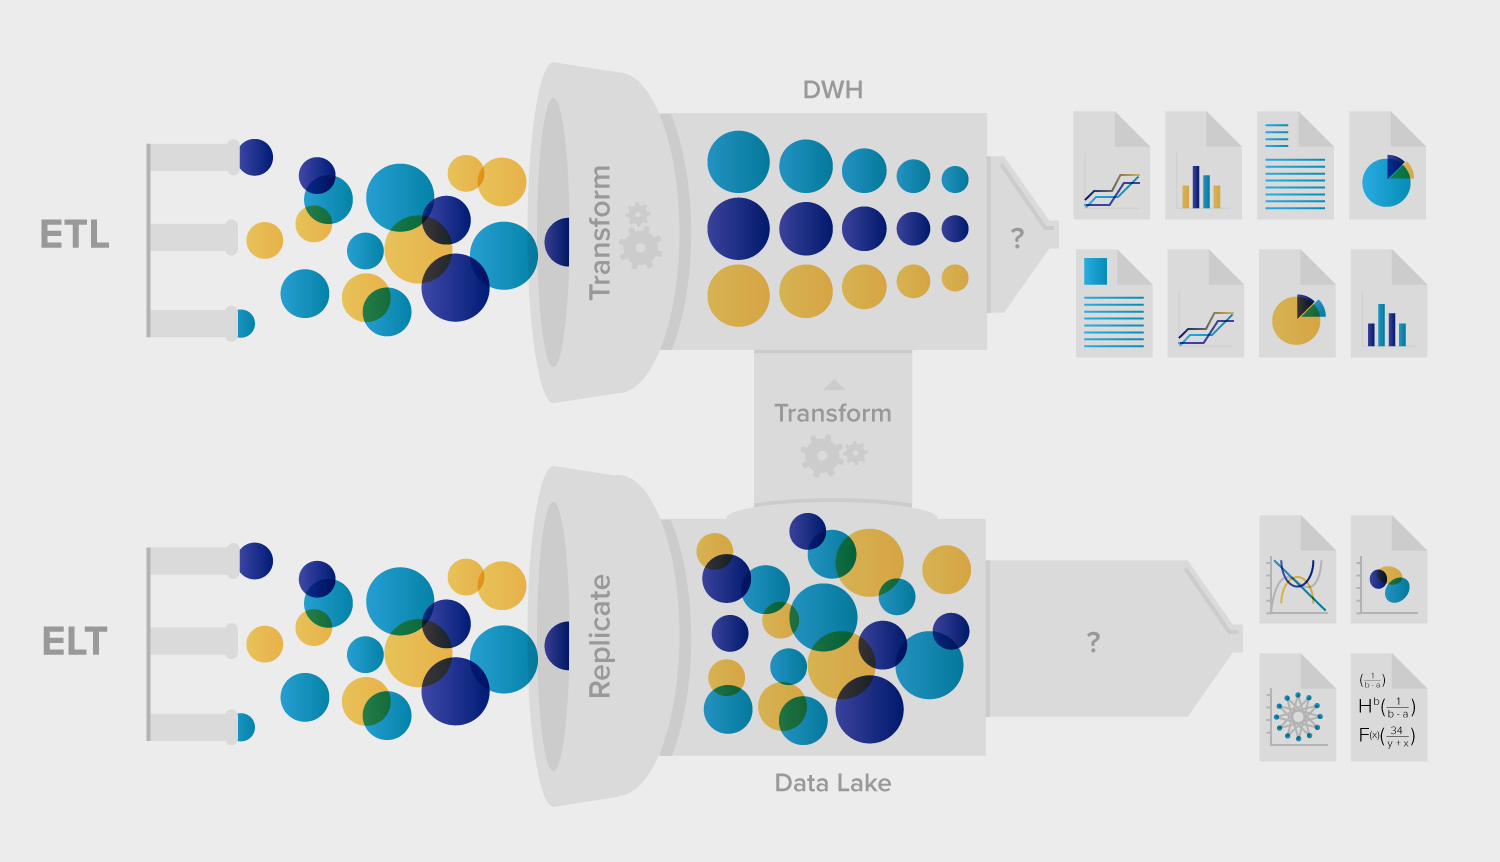
\includegraphics[width=1\linewidth]{images/ETL-ELT.png}
\small
\textit{Note.} The image depicts a comparison between two data processing approaches. ETL (Extract, Transform, Load) and ELT (Extract, Load, Transform). Both processes start with diverse data sources represented by colored circles; ETL transforms data before loading into a data warehouse (DWH); ELT loads data into a data lake first, then transforms it; The outcomes of both processes are visualized as various types of reports and charts
\textit{Creator:} (\cite{etleltDatacamp})\footnote[22]{\fullcite{etleltDatacamp}}
\end{figure}

\subsection{ETL (Extract, Transform, Load)}
\textbf{ETL} is a process where data is first extracted from source systems, then transformed into a consistent format and finally loaded into the target system (\cite{etleltDatacamp})\footnote[22]{\fullcite{etleltDatacamp}}.

\begin{itemize}
    \item In the \textbf{extraction phase}, data is gathered from several places during the extraction stage, including databases, files, APIs and streaming services. This phase entails managing many data formats, guaranteeing data consistency and resolving data quality problems; (\cite{etleltDatacamp})\footnotemark[22];
    \item To meet the destination system's schema, the extracted data is cleaned, validated and reorganized during the \textbf{transformation stage}. Data type conversions, data enrichment, data aggregation and the application of business rules or logic are all examples of data transformations that are often used (\cite{etleltDatacamp})\footnotemark[22];
    \item \textbf{Data is loaded} into the destination system — usually a data warehouse or data lake — after the transformation. This stage takes into account elements such data availability, integrity and volume (\cite{etleltDatacamp})\footnotemark[22].
\end{itemize}

When the destination system has limited processing power or the source data needs major modifications, ETL is often the better option. It makes complicated data transformations possible to be carried out prior to data loading, guaranteeing a consistent structure in the target system (\cite{etleltDatacamp})\footnotemark[22].

\subsection{ELT (Extract, Load, Transform)}
An other method called \textbf{ELT} loads the data straight into the target system once it has been retrieved from the source systems; the transformations take place after the loading procedures (\cite{etleltDatacamp})\footnotemark[22].

\begin{itemize}
    \item Like ETL, which gathers data from many sources and loads it into the target system, the \textbf{extraction and loading stages are comparable}. Nevertheless, the data is put in ELT in its original format without any previous processing (\cite{etleltDatacamp})\footnotemark[22];
    \item Utilising the processing power and capabilities of the target system, the \textbf{transformation phase} of ELT occurs there. Because the target system can effectively manage huge amounts of data, this enables more flexible and scalable data transformations (\cite{etleltDatacamp})\footnotemark[22].
\end{itemize}

Platforms for cloud computing and big data are making ELT more and more prevalent. Because transformations may be implemented on-demand depending on particular needs, it facilitates quicker data loading and more flexible data processing. ELT does, however, also bring difficulties like managing schema change in the destination system and guaranteeing data quality. Data integrity maintenance calls for strong data governance and data validation procedures (\cite{etleltDatacamp})\footnotemark[22].

\subsection{Comparison of ETL and ELT}
The complexity of data transformations, the processing power of the destination system and the particular needs of the data pipeline are only a few of the considerations when deciding between ETL and ELT. When the destination system is underpowered in processing or when the source data needs intricate changes, ETL is an option. In order to preserve both the quality and the integrity of the data, it guarantees that it is standardized before loading. Conversely, ELT works better with big amounts of data and when the destination system can handle it well enough. It makes data loading quicker and offers transformation application flexibility according to certain use cases (\cite{etleltDatacamp})\footnote[22]{\fullcite{etleltDatacamp}}.

\section{Data Security and Governance}

\textbf{Data security} — refers to the measures and practices implemented to protect data from unauthorized access, breaches, corruption and loss. In the context of data engineering, this involves securing data at rest, in transit and during processing.

\textbf{Data gowernance} — referes to the overall management of data availability, usability, integrity and security. The processes include establishing policies, procedures and standards for data management across the organization.

In today's business world, data has emerged as one of the most precious assets that companies possess. Accurate business insights and regulatory compliance depend on robustly controlling and managing data quality as data volumes increase dramatically across many platforms. Poor quality data may mask true insights and result in poor business choices (\cite{Achanta2023DataGA})\footnotemark[23]. In order to guarantee high-quality, safe and compliant data assets across the company, data governance offers the overall strategy, rules, standards and procedures. Through this process, regulatory, operational and strategic goals are brought into alignment with data management procedures. Important tasks include \textbf{creating data rules, standards and processes}; \textbf{controlling data models, metadata and quality};\textbf{ ensuring clear ownership and stewardship of data}; and \textbf{monitoring data usage and access for compliance and security} (\cite{Achanta2023DataGA})\footnotemark[23].

Core to governance is data security. Strong security measures must be implemented inside data platforms by enterprises in light of the increasing cybersecurity risks and stringent data protection laws like \textbf{GDPR}. This covers tools for data loss protection, activity monitoring, data encryption and finely tuned access controls. Standardization of data management and categorization guarantees sufficient protection of sensitive data (\cite{Achanta2023DataGA})\footnotemark[23]. Huge amounts of data go through many phases in data engineering pipelines, from ingestion to consumption. Governance and quality validations are crucially ingrained in data infrastructure and procedures by data engineers. Important areas of concentration include robust data validation during intake, data cleaning and standardization inside ETL processes, data quality checks in analytics and data lineage and cataloging (\cite{Achanta2023DataGA})\footnote[23]{\fullcite{Achanta2023DataGA}}.

\textbf{Absence of data governance results in data silos, erroneous data definitions, bad metadata and insufficient compliance}. Data exchange is hampered by this, which also damages data trust and raises regulatory concerns. Business, IT and compliance teams must be represented in the well-designed data governance architecture that is implemented. Definition of essential data items, reference data, data quality standards and data problem resolution need the establishment of procedures and responsibilities (\cite{Xie2021SolutionIA})\footnote[24]{\fullcite{Xie2021SolutionIA}}. New possibilities to scale governance are presented by emerging technology. Complicated data matching, quality assessment and anomaly detection may all be automated using machine learning. Tools for managing metadata provide impact analysis, data lineage and auto-classification. Users may find and comprehend data assets by using the business glossaries and data dictionaries included in data catalogs. Templates and procedures from cloud-based data governance providers help jumpstart projects (\cite{Achanta2023DataGA})\footnote[23]{\fullcite{Achanta2023DataGA}}.

\section{Real-World Data Security Challenges and Solutions}

The following subchapter is divided into four parts. The first part is a brief definition of the topic and the next three parts are example, challenge and solution, respectively.

\textbf{Encryption} — is the process of encoding data so that it can only be decoded with the right encryption key.

\begin{itemize}
    \item For instance, a financial services organization may utilize AES-256 encryption to safeguard private client data kept in its data warehouse. Data is encrypted in transit by the organization using TLS (Transport Layer Security) as it is transmitted between its on-premises systems and cloud-based analytics platforms.
    \item The problem is the advancements in quantum computing; there is increasing worry that these machines may be able to crack present encryption systems.
    \item Organizations looking to future-proof their data security are starting to investigate and use quantum-resistant encryption techniques, often referred to as post-quantum cryptography.
\end{itemize}

\textbf{Access control} —  Ensuring that only authorized personnel may access certain data sets requires the implementation of strong access control systems.

\begin{itemize}
    \item In their data lake, a healthcare provider may, for instance, use role-based access control (RBAC). All patient data may be available to doctors, but billing information is the only information administrative personnel may view. Anonymized data sets may be available to researchers.
    \item Controlling access permissions across many systems and platforms becomes more difficult as businesses expand and data is dispersed.
    \item A great solution are Identity and Access Management (IAM) systems that provide centralized management over user authentication and authorization across many systems and cloud platforms are being used by many companies. For access management that is both more granular and aware of the context, some people are also investigating the usage of attribute-based access control, often known as ABAC.
\end{itemize}

\textbf{Data masking and anonymization} — When sensitive data must be utilized for analytics or testing, data masking and anonymization methods are used to preserve data usefulness while safeguarding individual privacy.

\begin{itemize}
    \item A retail corporation may, for instance, utilize data masking methods to provide its marketing analytics team with consumer transaction data. The statistical features of the original dataset are preserved, while realistic but fictitious data replaces personally identifiable information (PII) such as names and addresses.
    \item Finding the appropriate equilibrium between the value of data and the preservation of privacy may be challenging, particularly when applied to more sophisticated re-identification systems.
    \item Differential privacy approaches are becoming more popular among firms. These techniques include the addition of noise to datasets that have been properly calibrated in order to give robust privacy assurances as well as the ability to do relevant analysis.
\end{itemize}

\textbf{Data catalog and metadata management}

\textbf{Metadata} — data that describes other data

\textbf{Data catalog} — centralized database that organizes and saves metadata on the data assets of an organization. It serves as an inventory system for data, providing information about data sources, schemas, relationships and usage.

\textbf{Metadata management} — is the process of creating, storing organizing and maintaining metadata.

\begin{itemize}
    \item An international company may, for instance, put in place a data catalog system that offers a searchable inventory of all data assets within the company. Information regarding the history of the data, its owners, measures of data quality and use rules is included in this catalog.
    \item Keeping an accurate and current data catalog is harder as data quantities and diversity rise.
    \item For automated data discovery and categorization, several companies are using machine learning and AI technology. These applications can identify data types, search data repositories automatically and update in real time the data catalog.
\end{itemize}

\textbf{Data quality management} — refers to the set of practices, processes and technologies used to measure, improve and maintain the quality of data within an organization

\begin{itemize}
    \item An online retailer may, for instance, include automatic data quality checks into their ETL processes. Among these checks might include validating that product pricing are within an expected range, verifying that client email addresses are formatted correctly and flagging any unusual spikes in order volumes that could be a sign of data problems.
    \item As data sources become more diverse and data volumes increase, maintaining consistent data quality becomes more complex.
    \item Numerous companies are using sophisticated data observability systems. These systems may automatically identify and notify on abnormalities across many data quality parameters and utilize machine learning to set baselines for data quality.
\end{itemize}

\textbf{Regulatory compliance} — refers to an organization's adherence to laws, regulations, guidelines and specifications relevant to its business processes. In data engineering and governance, refers to making sure that data management procedures, security protocols and privacy safeguards satisfy the criteria established by different regulatory agencies and business associations.

\begin{itemize}
    \item A worldwide bank must, for instance, abide by a number of laws, such as the California Consumer Protection Act (CCPA) and industry-specific rules like PCI DSS for payment card data. They implement compliance management system that monitors consent, data flows and offers audit trails for every data processing and accessing operation.
    \item New laws are established and current ones are amended on a regular basis, thus the regulatory environment is ever changing.
    \item To keep informed about regulatory changes, evaluate their effect and automate compliance procedures, many companies are using RegTech (Regulatory Technology) solutions that leverage AI and machine learning.
\end{itemize}

\textbf{Data ethics and responsible AI}

\begin{itemize}
    \item An AI ethics board that evaluates all AI projects is implemented by a big tech corporation that creates AI models for content recommendation. They also put into place methods to identify and reduce bias in their model outputs and training data.
    \item It may be difficult to define and apply moral principles for AI and data usage, particularly when addressing complicated situations or competing agendas.
    \item A few groups are embracing official guidelines for ethical AI, notably the EU's Ethics Guidelines for Trustworthy AI. When it comes to addressing ethical problems in the creation and deployment of artificial intelligence, these frameworks provide an organized approach.
\end{itemize}

\section{Data Serving}

Operating machine learning requires data pipelines to automate data flow from source to model training to inference. Because of shortcomings in the tools, the pipeline must smoothly combine stream processing with model serving for real-time applications. Particularly difficult is serving machine learning models on streaming data when the models must be updated often via online learning. Essential MLOps procedures include model versioning, monitoring, auditing and zero-downtime upgrades. In production, dynamic learning is made possible by scalable systems that use model serving frameworks and stream processing platforms like Kafka. The end-to-end latency and throughput are greatly influenced by the model serving setup's performance. Understanding the subtle variations between different streaming and serving technologies requires comparative benchmarking. For certain tasks, GPU-based hardware acceleration may be very beneficial. Semantic technologies are being used more and more to make building and using ML pipelines easier. Data science may be efficiently used by people who aren't ML specialists by capturing domain knowledge and ML best practices in ontologies. These ontologies can then be accessible via intelligent modules and intuitive interfaces. This has use in industrial environments (\cite{Cdola2021FeatureEA})\footnote[26]{\fullcite{Cdola2021FeatureEA}}.

\section{Monitoring and Maintenance}

Machine learning systems' foundation are data pipelines, which automate the flow of data from intake to model training and inference. The provision of machine learning models with timely and high-quality data to train from is made possible by a data pipeline that has been well-architected. It is important to monitor data flows so that problems are caught early and the system stays healthy generally. This includes tracking metrics on pipeline performance, data distribution, schema changes and data volume. Anomaly detection methods can be used to find quick changes and let engineers know about them. Considerable work is put into feature engineering and turning unprocessed data into features for machine learning models during pipeline construction. Combining transaction data, analyzing text sentiment, computing time-series statistics, etc. How well a model works depends a lot on how good its features are. Pipelines must be adaptable since data arrives in numerous forms from many sources. When dealing with unstructured data such as video, it may be necessary to use specific procedures. One example of this would be filtering video frames based on their quality and content in order to generate a training dataset that is representative. \textbf{Scalable data pipeline deployment has never been simpler thanks to cloud platforms}. So that data engineers may concentrate on pipeline logic, managed services take care of infrastructure provisioning and orchestration. Kubeflow is one tool that helps connect pipeline elements. Additionally, under active development is data versioning. Debugging and reproducibility of a certain model depend on the ability to monitor the version of data used to train it. Data lineage monitoring and pipeline metadata collecting make this possible. In conclusion, one of the most important applications of machine learning pipelines is the use of predictive maintenance in sectors such as manufacturing, energy and transportation. By analyzing sensor data and event records, models can anticipate equipment failures in advance, enabling the scheduling of restorations proactively. This enhances reliability and reduces costs. In conclusion, data pipeline seamless functioning depends on monitoring and maintenance, which in turn makes data-driven projects successful in many sectors. To keep the data flowing, proactive maintenance, careful monitoring and sound system design are all necessary (\cite{roychowdhury2021videodata}) \footnote[25]{\fullcite{roychowdhury2021videodata}}.